\subsection{GPIO}

\subsubsection{Introduction}

Simple peripheral with two 8bit input/outputs ports. Function is similar to AVR
GPIO ports, there is two register, DDR and PORT, logical one in DDR set this
pin as output, value written into right bit of PORT register will be on pin.
When logical zero in in DDR register, CPU can read values what are connected to
the pins through PORT register.

Whole architecture of GPIO is on picture \ref{fig:gpio_arch}. You can see four
registers, two pins I/O controllers and bus logic.

\begin{figure}[]
    \centering
    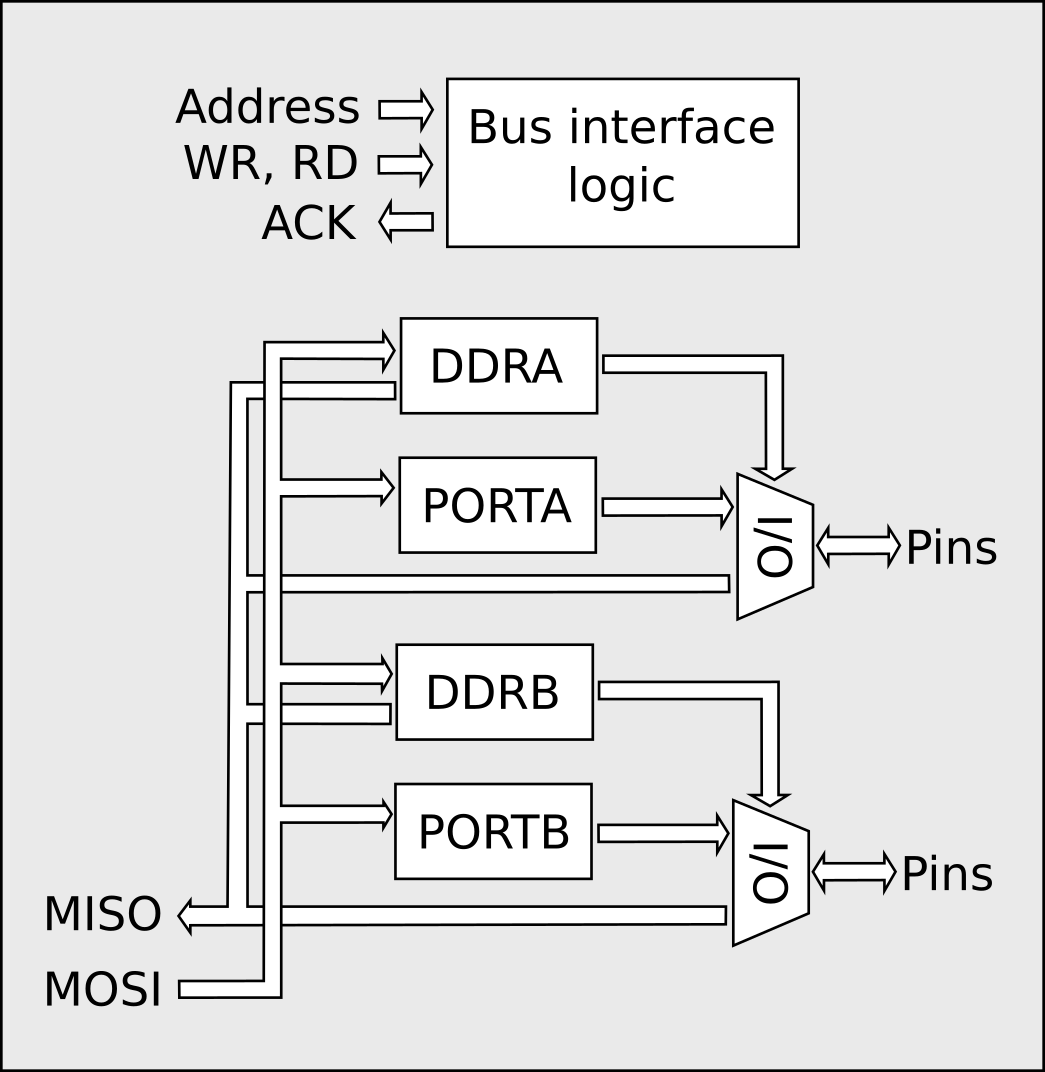
\includegraphics[width=.7\textwidth]{img/GPIO.png}
    \caption{GPIO architecture}
    \label{fig:gpio_arch}
\end{figure}

\subsubsection{Registers}

All registers are listed in table \ref{tab:gpio_reg_map}. Width of register are
equal to pins count (port width can be configured), by default it is 8
input/outputs. Meaning of seting in DDRx and PORTx registers are in table
\ref{tab:gpio_fuction}.

\begin{table}[]
    \centering
    \begin{tabular}{|l|l|l|}
        \hline
        \textbf{Offset} & \textbf{Name} & \textbf{Purpose}                                            \\ \hline
        $+0$            & PORTA         & Read from port A when input; write into port A when output. \\ \hline
        $+1$            & DDRA          & Set direction of PORTA                                      \\ \hline
        $+2$            & PORTB         & Read from port B when input; write into port B when output. \\ \hline
        $+3$            & DDRB          & Set direction of PORTB                                      \\ \hline
    \end{tabular}
    \caption{GPIO register map}
    \label{tab:gpio_reg_map}
\end{table}

\begin{table}[]
    \centering
    \begin{tabular}{|l|l|l|}
        \hline
        \textbf{DDRxx} & \textbf{PORTxx} & \textbf{Function}                               \\ \hline
        0              & 0               & Pin is in input mode.                           \\ \hline
        0              & 1               & Pin is in input mode.                           \\ \hline
        1              & 0               & Pin is in output mode, logical zero is written. \\ \hline
        1              & 1               & Pin is in output mode, logical one is written.  \\ \hline
    \end{tabular}
    \caption{GPIO function table}
    \label{tab:gpio_fuction}
\end{table}

\subsubsection{Hacking}

\begin{lstlisting}[language=VHDL, frame=single]
entity gpio is
    generic(
        BASE_ADDRESS: unsigned(23 downto 0) := x"000000";
        GPIO_WIDE: natural := 32
    );
    port(
        clk: in std_logic;
        res: in std_logic;
        address: in unsigned(23 downto 0);
        data_mosi: in unsigned(31 downto 0);
        data_miso: out unsigned(31 downto 0);
        WR: in std_logic;
        RD: in std_logic;
        ack: out std_logic;
        port_a: inout std_logic_vector((GPIO_WIDE-1) downto 0);
        port_b: inout std_logic_vector((GPIO_WIDE-1) downto 0)
    );
end entity gpio;
\end{lstlisting}

In listing abowe, you can see entity declaration of GPIO module, as you can see
you can very easily change size of GPIO with parameter GPIO\_WIDE. Base address
of GPIO can be changed too, with parameter BASE\_ADDRESS.

GPIO ports are inout ports "port\_a" and "port\_b". Other ports are used for
connecting to the system bus.

